\documentclass[12pt,a4paper]{article}

\usepackage[T2A]{fontenc}
\usepackage[utf8]{inputenc}
\usepackage[russian]{babel}
\usepackage{amsmath,amssymb}
\usepackage{graphicx}
\usepackage{geometry}
\usepackage{hyperref}
\geometry{margin=2.5cm}
\graphicspath{{figures/}}
\hypersetup{colorlinks=true,linkcolor=blue,urlcolor=blue}

\title{\textbf{Реализация PINN с использованием библиотек\\ Numpy и Numba (CUDA)}}
\author{Свиридов Никита}
\date{}

\begin{document}
\maketitle

\section{Введение}

PINN (Physics-Informed Neural Network) --- это нейросеть, предназначенная для
решения дифференциальных уравнений. Данную задачу можно считать обучением без
учителя, потому что для обучения такой сети не нужна разметка. Для расчёта
функции потерь используется само дифференциальное уравнение, а также граничные
и начальные условия.

Сеть обучается так, чтобы при подстановке функции, которую она задаёт, в наше
ДУ, ГУ и НУ отклонения от истинных значений были минимальны.

\section{Дифференциальное уравнение}

В качестве уравнения я взял уравнение теплопроводности --- уравнение в частных
производных до второго порядка:
\begin{equation*}
\begin{cases}
\dfrac{\partial u}{\partial t} = \Delta u + x\,t^2 \sin y, & 0 < x < 1,\ 0 < y < \tfrac{\pi}{2},\ t > 0,\\[2mm]
\dfrac{\partial u}{\partial x}\Big|_{x=0} = \dfrac{\partial u}{\partial x}\Big|_{x=1} = 0, & \\[2mm]
u\big|_{y=0} = 0, \quad \dfrac{\partial u}{\partial y}\Big|_{y=\pi/2} = 0, & \\[2mm]
u\big|_{t=0} = 0. &
\end{cases}
\end{equation*}

\section{Архитектура нейросети}

В качестве архитектуры выбран многослойный персептрон из 4 слоёв, между которыми
в качестве функции активации используется сигмоида:
\[
\sigma\!\big(\sigma(\sigma(X A_1 + B_1)A_2 + B_2)A_3 + B_3\big)A_4 + B_4,
\]
где $A_i$ --- матрица параметров слоя, $B_i$ --- свободный член (сложение
выполняется построчно), а
\[
\sigma(x) = \frac{1}{1 + e^{-x}}
\]
--- функция активации сигмоида. Для инициализации весов использован метод
Xavier: элементы матриц заполняются шумом из нормального распределения
$\mathcal{N}\!\big(0, 1/\dim_{\text{in}}\big)$.

\section{Реализация нейросети}

Можно выделить два этапа построения сети. Первый --- написание самого алгоритма
обучения. Второй --- перенос вычислений на CUDA.

\subsection{Алгоритм}

Нейросеть можно представить как большую параметризованную функцию. Обучение её
параметров, как и любой другой модели, основано на методе градиентного спуска:
разрабатывается функция потерь, в процессе обучения по ней вычисляется ошибка, а
затем --- градиенты параметров. Так как градиент указывает направление роста
функции, для минимизации ошибки параметры сдвигаются в сторону антиградиента.

Я предпочёл не выписывать формулы градиентов для слоёв вручную, а написать общий
вид сети и обучать уже её. Под общим видом подразумевается система
автоматического дифференцирования --- класс-обёртка (\texttt{tensor}) над
обычным тензором, который запоминает градиент по каждой арифметической операции
на каждом шаге вычислений. Благодаря этому всегда можно рассчитать градиент
любого элемента в графе вычислений методом обратного распространения ошибки.
Поскольку функции обратного прохода сами выражены через операции над тензорами,
граф градиентов тоже дифференцируем --- именно это позволяет брать производные
второго порядка ($u_{xx}$, $u_{yy}$), необходимые в уравнении.

\subsection{Параллельные вычисления}

Чтобы сеть работала за разумное время, вычисления перенесены на CUDA. При этом
нужно было решить проблему аллокации данных: обучение --- динамический процесс,
на каждом шаге вызываются сотни конструкторов и деструкторов нашего класса.
Переносить матрицы на видеокарту в момент обучения неэффективно. Поэтому заранее
выделяется большой блок памяти, в котором мы и работаем.

Я написал класс-обёртку над выделенной памятью \texttt{memory\_manager}, которому
делегируется задача выделения и очистки памяти в нашем массиве. Когда требуется
создать новый тензор, выбирается свободный участок и помечается как занятый;
когда вызывается деструктор --- участок снова становится доступным. Для выбора
участка используется жадный алгоритм минимизации фрагментации: свободные отрезки
поддерживаются в отсортированном по размеру виде, и поиск подходящего отрезка
выполняется за логарифмическое время бинарным поиском. При освобождении участок
сливается с соседними свободными отрезками.

Функции для распараллеливания можно разбить на три категории:
\begin{itemize}
  \item арифметические операции;
  \item заполнение памяти;
  \item reduce-операции.
\end{itemize}

\emph{Арифметические операции.} Реализованы: матричное произведение;
поэлементные сложение, умножение, деление, возведение в степень; поэлементное
вычисление $\ln$, $\cos$, $\sin$. В реализации матричного умножения используется
блочный (tiled) алгоритм с разделяемой памятью. Все бинарные операторы
определены и для случая, когда вторым аргументом является число.

\emph{Заполнение памяти.} Реализованы заполнение матрицы другой матрицей или
числом, взятие части матрицы по срезу и заполнение по срезу.

\emph{Reduce-операции.} Реализованы суммирование всех элементов, суммирование
вдоль оси столбцов и вдоль оси строк.

Все вычисления реализованы в двух взаимозаменяемых бэкендах: на чистом NumPy
(CPU) и на CUDA-ядрах (Numba). Граф автодифференцирования при этом один и тот
же.

\section{Обучение нейросети}

\emph{Функция ошибок.} Loss представляет собой сумму трёх типов слагаемых:
первое отвечает за выполнение дифференциального уравнения, второе --- за
граничные условия, третье --- за начальные:
\[
\text{Loss} = \Big\| \tfrac{\partial u_{\text{pinn}}}{\partial t} - \Delta u_{\text{pinn}} - x t^2 \sin y \Big\|
 + \sum_{i=1}^{4} \big\| \mathrm{BC}_i(u_{\text{pinn}}) \big\|
 + \big\| \mathrm{Init}(u_{\text{pinn}}) \big\|,
\]
где $\mathrm{BC}_i$ --- оператор граничных условий, $\mathrm{Init}$ --- оператор
начальных условий.

\emph{Параметры обучения.} Простое вычитание градиента не является наилучшим
решением, поэтому используется более продвинутый метод --- Adam. В моей
реализации применяется каноничный Adam с поправкой на смещение моментов
($\hat{m}$, $\hat{v}$). В качестве learning rate наиболее оптимальным оказалось
значение $0.01$; количество эпох выбрано равным $2000$ исходя из компромисса
между временем обучения и точностью решения.

\emph{Размер батчей в лосс-функциях.} На каждой эпохе случайным образом
генерируются точки из области, для которой ищется решение. Для ошибки ДУ точки
берутся из трёхмерного пространства $(x, y, t)$, а для НУ и ГУ одна из координат
фиксируется. Ошибка ДУ усредняется по $200$ точкам, а ошибки ГУ и НУ --- по
$50$ точкам каждая.

\section{Сравнение с аналитическим решением}

Аналитическое решение получено разделением переменных и разложением источника в
ряд Фурье по косинусам (удовлетворяющим условиям Неймана по $x$) и по $\sin y$
(удовлетворяющему условиям по $y$). Максимальное абсолютное отклонение численного
решения от аналитического не превышает $\approx 0.01$ при $t = 1$.

\begin{figure}[h]
\centering
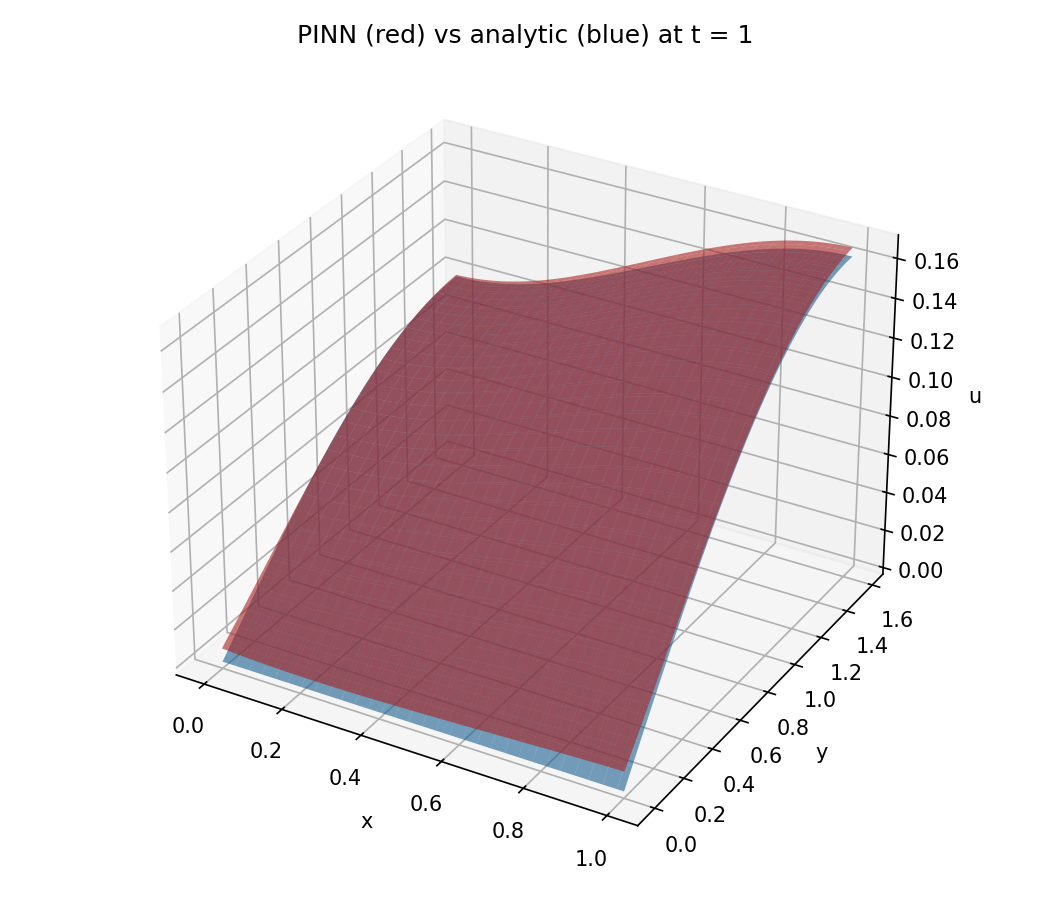
\includegraphics[width=0.48\textwidth]{comparison_t1.png}
\hfill
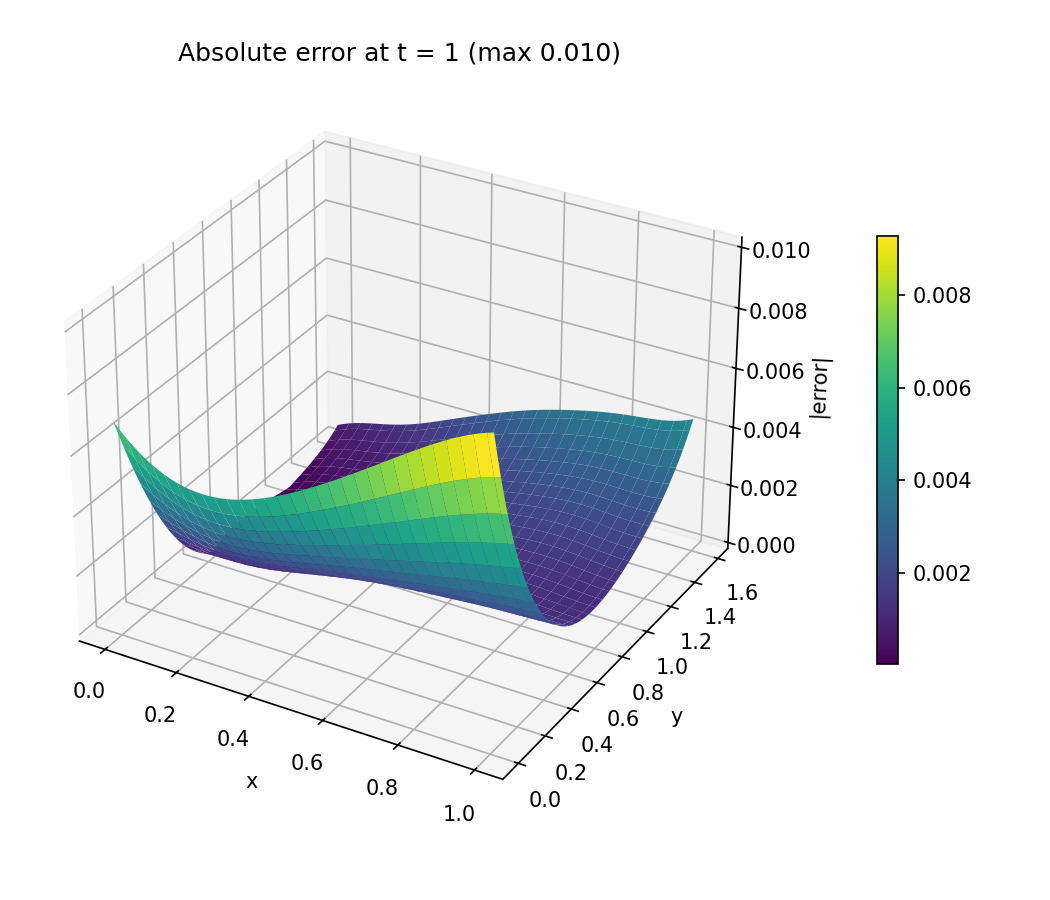
\includegraphics[width=0.48\textwidth]{error_field.png}
\caption{Слева: сравнение с аналитическим решением (синим --- аналитическое,
красным --- численное). Справа: поле абсолютной ошибки при $t = 1$.}
\end{figure}

\begin{figure}[h]
\centering
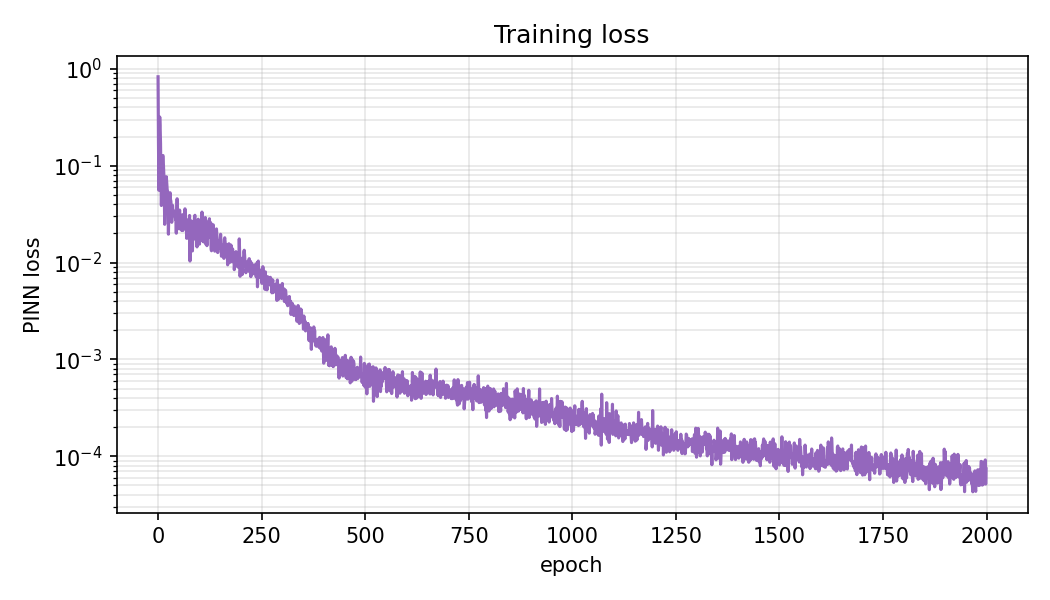
\includegraphics[width=0.7\textwidth]{loss_curve.png}
\caption{Кривая функции потерь в процессе обучения (логарифмическая шкала).}
\end{figure}

Говоря об актуальности решения ДУ с помощью PINN, отмечу, что данный подход
способен составить конкуренцию другим численным методам решения ДУ: при
использовании библиотечных реализаций количество эпох может быть существенно
увеличено, а точность --- повышена на порядки.

\section{Производительность}

Было проведено сравнение автоматического дифференцирования при вычислениях на
CUDA и на обычном NumPy. На малых размерах матриц, используемых в данной
архитектуре (ни по одной оси размер не превышает нескольких сотен), видеокарта
недозагружена, поэтому основной накладной расход --- это не сами вычисления, а
оркестрация: тысячи запусков мелких ядер на каждой эпохе и граф
автодифференцирования, построенный из Python-объектов. Это же объясняет, почему
самописная реализация медленнее PyTorch: его диспетчеризация и граф реализованы
на C++, а операции сливаются (fusion). Таким образом, узким местом является не
язык ядра, а оркестрация и размер задачи.

\end{document}
